\section{Optimization \& SGD}
\subsection{MSE as Function}

\subsection{Gradient Descent}


\begin{minipage}{0.5\linewidth}
    \begin{center}
        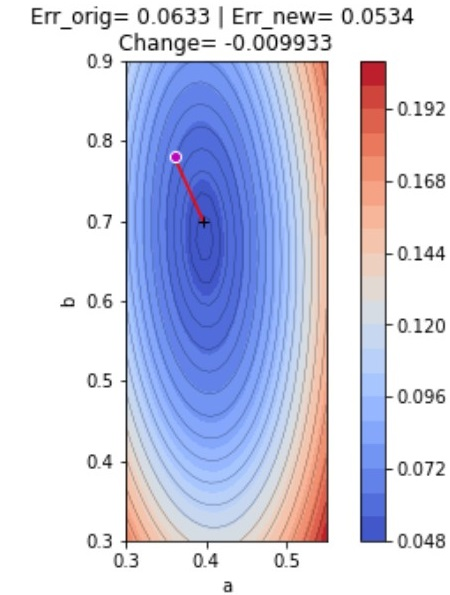
\includegraphics[width=\linewidth]{gradient-moving.jpg}
        \vspace{-8pt}
    \end{center}
\end{minipage}
\begin{minipage}{0.45\linewidth}
    \textbf{An iterative method}.\\
    At each iteration, the model parameters are updated such that the Loss (MSE) is reduced.
    At any location [a,b] move a step in the direction where the error shrinks the most.\\
\end{minipage}

\subsubsection{Calculation}
\textbf{MSE Formula:}
\begin{center}
    $E = \frac{1}{2N} * \large\displaystyle\sum_{i = 1}^{N}(\hat{y_i} - (a*x_i + b))^2$
\end{center}
\textbf{Gradient of E:}
\begin{center}
    $
        E = \left[\begin{array}{c} \frac{\partial E}{\partial a} \\ \frac{\partial E}{\partial b} \end{array}\right]
        = \left[\begin{array}{c} \frac{1}{N} \sum_{i=1}^N (y_i - (a * x_i + b))(-x_i) \\ \frac{1}{N} \sum_{i=1}^N (y_i - (a * x_i + b))(-1) \end{array}\right]
    $
\end{center}

\subsubsection{Update Rule}
\begin{align}
   \begin{bmatrix}
           a \\
           b \\
         \end{bmatrix}_{t+1} 
         =    \begin{bmatrix}
           a \\
           b \\
         \end{bmatrix}_{t} - \alpha 
         \begin{bmatrix}
           \frac{\partial E}{\partial a} \\
           \frac{\partial E}{\partial b} \\
         \end{bmatrix} \Big\rvert _{\begin{bmatrix}
           a \\
           b \\
         \end{bmatrix}_{t} }
  \end{align}
\\
The algorithm starts at some initial position $[a, b]_{t0}$. 
Then, the update rule is applied repeatedly. 
The number of update steps needed to come ``close enough'' to the minimum depends on the problem.

\subsection{Stochastic Gradient Descent (SGD)}
\begin{itemize}
    \item At each iteration, the gradient is calculated on a (randomly selected) subset of the data
    \item For a fixed learning rate, SGD does not converge
\end{itemize}

\subsubsection{Annealed SGD}
\begin{itemize}
    \item The learning rate alpha is reduced over time
    \item This is called (simulated) annealing
    \item There are different options (called schedules) how to reduce alpha over time
\end{itemize}

\subsubsection{General remarks on SGD}
\begin{itemize}
    \item Gradient-based methods only work if we can express a Loss function as a differentiable function
    \item SGD is dealing woth only a single datum at each iteration. This is very inefficient and rarely used.
    \item Batch- or mini-batch gradient-descent is usually used
\end{itemize}